\documentclass[aps,prb,onecolumn,superscriptaddress,floatfix]{revtex4-2}
\usepackage{amsmath,amssymb,bm}
\usepackage{graphicx}
\usepackage{booktabs}
\usepackage{xcolor}
\usepackage[colorlinks=true,allcolors=blue!50!black]{hyperref}
\renewcommand{\thetable}{S\arabic{table}}
\renewcommand{\thefigure}{S\arabic{figure}}
\renewcommand{\thesection}{S\arabic{section}}
\renewcommand{\theequation}{S\arabic{equation}}

\renewcommand{\figurename}{Figure}
\renewcommand{\tablename}{Table}
\renewcommand{\thetable}{\arabic{table}}
\begin{document}

\title{Supplemental Material for ``Local-resolvent formulation and assessment of linear-scaling Kohn--Sham calculations''}
\author{Albert Linda}
\affiliation{Department of Materials Science and Engineering, Indian Institute of Technology Kanpur,
Kanpur 208016, Uttar Pradesh, India}
\date{\today}
\maketitle

This Supplemental Material gives the data behind statements in the main text that are not shown there in full. All
numbers are generated by the scripts listed in Section~\ref{sec:repro} from the files in \texttt{results/}. Lemma,
Proposition, Theorem and Remark numbers refer to the main text.

% =============================================================================
\section{Kohn--Sham reference solvers}\label{sec:ks}
% =============================================================================

\paragraph*{Dense solvers.} We compared three LAPACK paths for the dense generalized eigenproblem, and two ways of building
the density from the eigenvectors (Table~\ref{tab:ksdrivers}). The paths were \texttt{dsygvx} (bisection and inverse
iteration for the lowest $N/2+1$ pairs), \texttt{dsygvd} (divide and conquer, all pairs), and Cholesky reduction with
\texttt{dsyevr} (MRRR, the lowest $N/2+1$ pairs). The density was built either as the orbital sum
$2\sum_i|\sum_\mu X_{\bm r\mu}C_{\mu i}|^2$ or by projecting $P=2CC^{\mathsf T}$ (formed with \texttt{dsyrk}) through the sparse
basis. The six variants give the same density. The automated test asserts agreement to $10^{-10}$, and the observed
differences are of order $10^{-15}$.

For 432 electrons and more the eigensolver takes more than 84\% of the time. For 128
electrons it takes about 40\%, and building the density takes 8\% (orbital sum) to 19\% (density matrix).
\texttt{dsygvx} and \texttt{dsyevr} are equally fast and \texttt{dsygvd} is slower; we use \texttt{dsygvx} with the orbital
sum. In 1D, bisection (\texttt{stebz}) with inverse iteration was faster than MRRR (\texttt{stemr}) for the occupied states
of dimerized chains (Table~\ref{tab:ks1d}).

\paragraph*{Warm-started LOBPCG.} As an iterative reference we used LOBPCG on the pencil $(H,S)$, with $N/2+24$ vectors, a
block-Jacobi preconditioner $(H-\sigma S)^{-1}$ with one block per molecule and $\sigma$ 0.5~Ha below the lowest eigenvalue,
and starting vectors from the previous SCF step. The first step is solved densely. Table~\ref{tab:lobpcg} shows that it is
slower than dense diagonalization at all sizes tested, with up to 63 LOBPCG iterations per SCF step. At 1024 electrons a warm
LOBPCG step took about 46~s, against 38~s for a dense step.

\begin{table}[h]
\caption{\label{tab:ksdrivers}3D dense KS density build (s, single thread, best of 2--3): eigensolver time, density time and
total.}
\begin{ruledtabular}
\begin{tabular}{rrllrrr}
$N$ & $N_b$ & driver & density & eigensolver & density & total \\
\hline
128 & 768 & \texttt{gvx} & orbitals & 0.06 & 0.01 & 0.15 \\
128 & 768 & \texttt{gvx} & DM & 0.06 & 0.03 & 0.17 \\
128 & 768 & \texttt{gvd} & orbitals & 0.11 & 0.01 & 0.20 \\
128 & 768 & \texttt{gvd} & DM & 0.11 & 0.03 & 0.21 \\
128 & 768 & \texttt{evr} & orbitals & 0.06 & 0.01 & 0.15 \\
128 & 768 & \texttt{evr} & DM & 0.06 & 0.03 & 0.17 \\
432 & 2592 & \texttt{gvx} & orbitals & 2.44 & 0.15 & 2.89 \\
432 & 2592 & \texttt{gvx} & DM & 2.45 & 0.16 & 2.91 \\
432 & 2592 & \texttt{gvd} & orbitals & 4.21 & 0.15 & 4.67 \\
432 & 2592 & \texttt{gvd} & DM & 4.21 & 0.16 & 4.67 \\
432 & 2592 & \texttt{evr} & orbitals & 2.45 & 0.15 & 2.91 \\
432 & 2592 & \texttt{evr} & DM & 2.45 & 0.16 & 2.91 \\
1024 & 6144 & \texttt{gvx} & orbitals & 36.19 & 1.25 & 38.33 \\
1024 & 6144 & \texttt{gvx} & DM & 36.11 & 0.79 & 37.98 \\
1024 & 6144 & \texttt{gvd} & orbitals & 60.92 & 1.18 & 63.44 \\
1024 & 6144 & \texttt{gvd} & DM & 60.57 & 0.79 & 62.56 \\
1024 & 6144 & \texttt{evr} & orbitals & 36.40 & 1.18 & 38.86 \\
1024 & 6144 & \texttt{evr} & DM & 36.47 & 0.79 & 38.45 \\

\end{tabular}
\end{ruledtabular}
\end{table}

\begin{table}[h]
\caption{\label{tab:ks1d}1D tridiagonal KS solvers for the occupied states (s, best of 2).}
\begin{ruledtabular}
\begin{tabular}{rrrr}
$N$ & $N_g$ & \texttt{stebz} & \texttt{stemr} \\
\hline
256 & 5763 & 0.233 & 0.878 \\
512 & 11395 & 1.255 & 3.117 \\
1024 & 22659 & 8.188 & 10.897 \\

\end{tabular}
\end{ruledtabular}
\end{table}

\begin{table}[h]
\caption{\label{tab:lobpcg}Complete SCF calculations with warm-started LOBPCG and with dense KS: tolerance of LOBPCG, SCF
iterations, energy difference to dense KS per electron, wall times (s), and the largest number of LOBPCG iterations in one
SCF step.}
\begin{ruledtabular}
\begin{tabular}{rrrrrrr}
$N$ & tol & SCF it. & $|\Delta E|/N$ & LOBPCG wall & dense wall & max.\ LOBPCG it. \\
\hline
128 & 1e-05 & 11 & $5.5\times10^{-11}$ & 3.2 & 2.0 & 63 \\
128 & 1e-07 & 11 & $8.4\times10^{-14}$ & 4.3 & 2.0 & 63 \\
432 & 1e-05 & 11 & $9.0\times10^{-11}$ & 43.8 & 34.3 & 63 \\
432 & 1e-07 & 11 & $4.6\times10^{-13}$ & 66.9 & 34.3 & 63 \\

\end{tabular}
\end{ruledtabular}
\end{table}

% =============================================================================
\section{Timing methodology, repeatability and threads}
% =============================================================================

All timings are wall-clock times measured with \texttt{time.perf\_counter} on an 8-core workstation (Linux, OpenBLAS
0.3.26).

\paragraph*{Complete SCF calculations.} Table~\ref{tab:rigorousall} lists every run behind the SCF wall times of the main
text (protocol: main text, Computational details, Timing). Both methods needed
the same number of SCF iterations at each size. The 2000-electron LRes-DFT value is a single run.

\begin{table}[h]
\caption{\label{tab:rigorousall}Wall time (s) of every complete SCF calculation, in run order (single thread, idle machine).}
\begin{ruledtabular}
\begin{tabular}{rllc}
$N$ & KS & LRes-DFT & SCF it. \\
\hline
54 & 0.5, 0.6, 0.5 & 3.2, 3.3, 3.2 & 11 \\
128 & 2.0, 1.9, 1.9 & 8.6, 8.9, 8.4 & 11 \\
250 & 7.4, 7.2, 7.1 & 25.2, 24.7, 25.0 & 11 \\
432 & 35.2, 34.6, 33.9 & 46.5, 46.0, 44.6 & 11 \\
686 & 136.5, 132.0, 131.4 & 65.4, 66.4, 65.8 & 11 \\
1024 & 445.1, 441.2, 442.9 & 126.0, 125.0, 125.4 & 11 \\
2000 & -- & 272.1 & 11 \\
\end{tabular}
\end{ruledtabular}
\end{table}

\paragraph*{Density builds.} For LRes-DFT, the warm step reuses $\mu$ and $E_\mathrm{lo}$ from a previous call and computes only
window eigenpairs below $c+1.5R$. The cold step computes all window eigenvalues, determines $\mu$, and then builds the
density. The window vectors on the owned points are stored, so re-solving $\mu$ in a warm step needs no second eigensolver
pass. The density-build series of the main text was measured on a shared machine at a load average near 1 (best of 2--3).
Table~\ref{tab:repeat} shows a separate series of five repetitions taken earlier under heavier load. There the standard
deviations reached 12\% (432 electrons) and 20\% (686 electrons) for KS and up to 10\% for LRes-DFT. This is why the main
text uses complete SCF calculations on an idle machine for the headline comparison. Table~\ref{tab:threads} gives
shared-memory timings at 432 electrons (load average 1--3): OpenMP over windows for LRes-DFT, and threaded OpenBLAS for KS.

\begin{table}[h]
\caption{\label{tab:repeat}Repeatability under load: mean and standard deviation (s) of five density builds.}
\begin{ruledtabular}
\begin{tabular}{rrrrr}
$N$ & KS mean & KS s.d. & LRes-DFT mean & LRes-DFT s.d. \\
\hline
250 & 0.620 & 0.004 & 1.647 & 0.010 \\
432 & 3.455 & 0.415 & 2.834 & 0.122 \\
686 & 13.510 & 2.679 & 4.628 & 0.447 \\

\end{tabular}
\end{ruledtabular}
\end{table}

\begin{table}[h]
\caption{\label{tab:threads}Shared-memory threads, 432 electrons (s, best of 3).}
\begin{ruledtabular}
\begin{tabular}{rrrr}
threads & LRes-DFT warm step & KS & load average \\
\hline
1 & 2.66 & 2.90 & 0.8 \\
2 & 1.54 & 2.26 & 1.0 \\
4 & 1.16 & 2.59 & 1.5 \\
8 & 0.97 & 2.72 & 2.6 \\

\end{tabular}
\end{ruledtabular}
\end{table}

\begin{table}[h]
\caption{\label{tab:cost1d}1D cost data (s): LRes-DFT with the exact recursion including the search for $\mu$ from scratch,
one LRes-DFT evaluation at fixed $\mu$, the window variant, the tridiagonal KS solver and dense KS, and the window error per
electron.}
\begin{ruledtabular}
\begin{tabular}{rrrrrrrr}
$N$ & $N_g$ & LRes-DFT & LRes-DFT, fixed $\mu$ & windows & KS (stebz) & KS (dense) & window error \\
\hline
16 & 483 & 0.014 & 0.0004 & 0.035 & 0.001 & 0.02 & $0$ \\
32 & 835 & 0.020 & 0.0008 & 0.064 & 0.004 & 0.07 & $4.1\times10^{-8}$ \\
64 & 1539 & 0.058 & 0.0013 & 0.265 & 0.021 & 1.83 & $1.3\times10^{-7}$ \\
128 & 2947 & 0.127 & 0.0027 & 0.328 & 0.056 & 10.58 & $1.5\times10^{-7}$ \\
256 & 5763 & 0.361 & 0.0086 & 1.211 & 0.621 & 80.45 & $1.5\times10^{-7}$ \\
512 & 11395 & 0.729 & 0.0167 & 2.525 & 3.190 & -- & $1.6\times10^{-7}$ \\
1024 & 22659 & 0.858 & 0.0217 & 3.437 & 22.733 & -- & $1.6\times10^{-7}$ \\
2048 & 45187 & 1.749 & 0.0449 & 5.661 & 216.198 & -- & $1.6\times10^{-7}$ \\
4096 & 90243 & 4.281 & 0.1164 & 18.224 & -- & -- & $1.6\times10^{-7}$ \\
8192 & 180355 & 9.762 & 0.2604 & nan & -- & -- & -- \\

\end{tabular}
\end{ruledtabular}
\end{table}

% =============================================================================
\section{Memory}
% =============================================================================

The peak resident memory of the solver step was measured by resetting the peak counter of the process after the basis,
grid, Hamiltonian and window index data had been built (\texttt{/proc/self/clear\_refs}). The high-water mark
(\texttt{VmHWM}) was then read after the step (Table~\ref{tab:mem}). The LRes-DFT process holds an additional 86~MB of
window index data at 1024 electrons, which is not included in the step memory. The LRes-DFT step memory grows faster than
linearly in this range because it includes the stored window vectors and per-window work arrays.

\begin{table}[h]
\caption{\label{tab:mem}Memory of one density build (MB): resident memory before the step and additional peak memory of the
step.}
\begin{ruledtabular}
\begin{tabular}{rrlrr}
$N$ & $N_b$ & method & before & additional peak \\
\hline
128 & 768 & LR-DFT & 168 & 21 \\
128 & 768 & KS & 165 & 21 \\
250 & 1500 & LR-DFT & 251 & 39 \\
250 & 1500 & KS & 248 & 28 \\
432 & 2592 & LR-DFT & 341 & 83 \\
432 & 2592 & KS & 338 & 112 \\
686 & 4116 & LR-DFT & 494 & 130 \\
686 & 4116 & KS & 491 & 271 \\
1024 & 6144 & LR-DFT & 666 & 251 \\
1024 & 6144 & KS & 580 & 676 \\

\end{tabular}
\end{ruledtabular}
\end{table}

% =============================================================================
\section{Basis set and window error}
% =============================================================================

Table~\ref{tab:basis} compares three bases:
\begin{itemize}
\item compact: five functions per atom, $s$ exponents 1.0 and 0.25, $p$ exponent 0.6~bohr$^{-2}$, cutoff 4.5~bohr;
\item the basis used in the main text: $s$ exponents 1.2, 0.4 and 0.15, $p$ exponent 0.5, cutoff 4.5~bohr;
\item diffuse: $s$ exponents 1.0, 0.3 and 0.12, $p$ exponent 0.5, cutoff 5.5~bohr.
\end{itemize}
The basis error is the difference between the LCAO-KS and real-space-grid KS energies for a 16-electron crystal. The window
error is the LRes-DFT--KS difference at the self-consistent potential of a 250-electron crystal. A more complete, more
diffuse basis lowers the basis error but raises the window error.

\begin{table}[h]
\caption{\label{tab:basis}Basis-set trade-off.}
\begin{ruledtabular}
\begin{tabular}{lrrrrrr}
basis & basis error/$N$ (Ha) & $\lambda_\mathrm{min}(S)$ & $R_w$ & $n_W$ & $\|\Delta n\|_1/N$ & $|\Delta E_\mathrm{band}|/N$ \\
\hline
compact (5 per atom, $r_c=4.5$~bohr) & 0.0505 & 0.0252 & 8.5 & 190 & $1.2\times10^{-5}$ & $1.9\times10^{-7}$ \\
compact (5 per atom, $r_c=4.5$~bohr) & 0.0505 & 0.0252 & 12.1 & 330 & $1.3\times10^{-7}$ & $8.5\times10^{-9}$ \\
used (6 per atom, $r_c=4.5$~bohr) & 0.0188 & 0.0068 & 8.5 & 228 & $1.0\times10^{-4}$ & $2.0\times10^{-6}$ \\
used (6 per atom, $r_c=4.5$~bohr) & 0.0188 & 0.0068 & 12.1 & 396 & $3.6\times10^{-6}$ & $1.5\times10^{-7}$ \\
diffuse (6 per atom, $r_c=5.5$~bohr) & 0.0047 & 0.0040 & 8.5 & 228 & $5.9\times10^{-4}$ & $7.2\times10^{-5}$ \\
diffuse (6 per atom, $r_c=5.5$~bohr) & 0.0047 & 0.0040 & 12.1 & 396 & $3.8\times10^{-5}$ & $4.8\times10^{-6}$ \\

\end{tabular}
\end{ruledtabular}
\end{table}

% =============================================================================
\section{Pole rules: margin, error bound, closing gap and occupation range (1D)}
% =============================================================================

Table~\ref{tab:margin} and Figure~\ref{fig:sm}(b) show the density error of the (H$_2$)$_{16}$ chain as a function of the
margin $\delta$, with the rate $\rho$ of Theorem~1. The per-state bound $\rho^M$ in that table is multiplied by an estimate
$2(N_\mathrm{occ}+5)/N$, so it is only indicative. The full bound of Theorem~1, evaluated exactly as stated, is given in
Table~\ref{tab:bound} and plotted in Figure~3(a) of the main text. Table~\ref{tab:gap} gives the number of poles needed for
uniform H chains whose gap closes with length. Table~\ref{tab:occ} gives the range of the occupations of the
Gauss--Legendre and Zolotarev rules at the order needed for $10^{-6}$ accuracy. The half-step rule stays within $[0,1]$ in
all cases.

\begin{table}[h]
\caption{\label{tab:margin}Margin $\delta$ (Ha): rate $\rho$, measured density error per electron and indicative bound.}
\begin{ruledtabular}
\begin{tabular}{rrrrr}
$\delta$ & $M$ & $\rho$ & error/$N$ & bound/$N$ \\
\hline
0.02 & 32 & 0.860 & $1.1\times10^{-3}$ & $1.1\times10^{-2}$ \\
0.02 & 48 & 0.860 & $8.9\times10^{-5}$ & $9.5\times10^{-4}$ \\
0.05 & 32 & 0.684 & $6.4\times10^{-7}$ & $6.8\times10^{-6}$ \\
0.05 & 48 & 0.684 & $1.4\times10^{-9}$ & $1.5\times10^{-8}$ \\
0.1 & 32 & 0.666 & $2.1\times10^{-7}$ & $3.0\times10^{-6}$ \\
0.1 & 48 & 0.666 & $2.7\times10^{-10}$ & $4.5\times10^{-9}$ \\
0.2 & 32 & 0.718 & $2.3\times10^{-6}$ & $3.2\times10^{-5}$ \\
0.2 & 48 & 0.718 & $1.0\times10^{-8}$ & $1.6\times10^{-7}$ \\
0.3 & 32 & 0.755 & $1.3\times10^{-5}$ & $1.7\times10^{-4}$ \\
0.3 & 48 & 0.755 & $1.2\times10^{-7}$ & $1.9\times10^{-6}$ \\
0.5 & 32 & 0.807 & $1.1\times10^{-4}$ & $1.4\times10^{-3}$ \\
0.5 & 48 & 0.807 & $3.1\times10^{-6}$ & $4.4\times10^{-5}$ \\
1.0 & 32 & 0.873 & $1.6\times10^{-3}$ & $1.7\times10^{-2}$ \\
1.0 & 48 & 0.873 & $1.6\times10^{-4}$ & $2.0\times10^{-3}$ \\
2.0 & 32 & 0.925 & $1.4\times10^{-2}$ & $1.0\times10^{-1}$ \\
2.0 & 48 & 0.925 & $3.3\times10^{-3}$ & $3.1\times10^{-2}$ \\

\end{tabular}
\end{ruledtabular}
\end{table}

\begin{table}[h]
\caption{\label{tab:bound}Theorem~1 for the (H$_2$)$_{16}$ chain ($\delta=0.3$~Ha): total $L_1$ density error, error per
electron, and the bound $2(N_\mathrm{occ}+N_\mathrm{near})\rho^M+2N_g2^{-M}$.}
\begin{ruledtabular}
\begin{tabular}{rrrr}
$M$ & $\|n_M-n\|_1$ & per electron & bound \\
\hline
8 & $5.7\times10^{-1}$ & $1.8\times10^{-2}$ & $1.2\times10^{1}$ \\
16 & $4.6\times10^{-2}$ & $1.4\times10^{-3}$ & $5.6\times10^{-1}$ \\
24 & $4.2\times10^{-3}$ & $1.3\times10^{-4}$ & $5.7\times10^{-2}$ \\
32 & $4.0\times10^{-4}$ & $1.3\times10^{-5}$ & $6.0\times10^{-3}$ \\
48 & $3.9\times10^{-6}$ & $1.2\times10^{-7}$ & $6.8\times10^{-5}$ \\
64 & $4.0\times10^{-8}$ & $1.3\times10^{-9}$ & $7.6\times10^{-7}$ \\
96 & $4.5\times10^{-12}$ & $1.4\times10^{-13}$ & $9.6\times10^{-11}$ \\
128 & $3.0\times10^{-15}$ & $9.3\times10^{-17}$ & $1.2\times10^{-14}$ \\

\end{tabular}
\end{ruledtabular}
\end{table}

\begin{table}[h]
\caption{\label{tab:gap}Uniform H$_n$ chains (spacing 2~bohr): gap and number of poles $M$ needed for density errors of
$10^{-4}$ and $10^{-6}$ per electron (half-step rule, $\delta=0.3$~Ha).}
\begin{ruledtabular}
\begin{tabular}{rrrr}
$n$ & gap (Ha) & $M$ ($10^{-4}$) & $M$ ($10^{-6}$) \\
\hline
10 & 0.095 & 50 & 82 \\
20 & 0.052 & 80 & 136 \\
40 & 0.027 & 134 & 238 \\
80 & 0.014 & 228 & 426 \\

\end{tabular}
\end{ruledtabular}
\end{table}

\begin{table}[h]
\caption{\label{tab:occ}Occupation range of the Gauss--Legendre (GL) and Zolotarev rules at the order needed for $10^{-6}$:
minimum occupation and maximum minus one.}
\begin{ruledtabular}
\begin{tabular}{lrrrrr}
case & gap (Ha) & GL min & GL max$-1$ & Zolotarev min & Zolotarev max$-1$ \\
\hline
H10 chain & 0.095 & -2.1e-07 & 5.5e-12 & -3.0e-07 & 2.3e-07 \\
H20 chain & 0.052 & -1.2e-05 & 3.3e-06 & -7.5e-07 & 7.2e-07 \\
H40 chain & 0.027 & -2.4e-05 & 1.7e-05 & -7.2e-07 & 7.2e-07 \\
H80 chain & 0.014 & -8.0e-08 & 8.1e-08 & -1.7e-06 & 1.7e-06 \\
core Z=4 & 0.107 & -5.7e-06 & 3.3e-07 & -6.8e-07 & 6.0e-07 \\
core Z=8 & 0.045 & -8.0e-06 & 6.6e-06 & -9.2e-07 & 8.4e-07 \\

\end{tabular}
\end{ruledtabular}
\end{table}

% =============================================================================
\section{Grid refinement against a Chebyshev expansion}
% =============================================================================

For an (H$_2$)$_4$ chain, Table~\ref{tab:grid} compares the number of poles $M$ of the half-step rule with the degree of a
Chebyshev interpolant of a Fermi function needed for a density error of $10^{-6}$ per electron. The smearing of the Fermi
function was chosen so that its own error is below the target, which requires a small temperature and a high degree. A
damped polynomial approximant of the gapped step would need a lower degree. A polynomial term also costs one matrix--vector
product, while a pole costs one linear solve. The comparison therefore shows only that the pole count does not depend on the
grid spacing while the polynomial degree does; it is not a cost comparison.

\begin{table}[h]
\caption{\label{tab:grid}Grid refinement at fixed gap.}
\begin{ruledtabular}
\begin{tabular}{rrrrrr}
$\Delta x$ & $N_g$ & $W$ (Ha) & $\Delta$ (Ha) & $M$ & Chebyshev degree \\
\hline
0.2 & 134 & 50 & 0.232 & 36 & 1792 \\
0.1 & 267 & 200 & 0.233 & 36 & 3648 \\
0.05 & 533 & 800 & 0.233 & 36 & 6144 \\
0.025 & 1065 & 3200 & 0.233 & 36 & 12288 \\

\end{tabular}
\end{ruledtabular}
\end{table}

% =============================================================================
\section{Pointwise probing on a real-space grid}
% =============================================================================

Table~\ref{tab:probing} documents the abandoned 3D route. For a two-molecule H$_2$ cell on a 0.6~bohr grid, we compare the
probed diagonal of the exact density matrix, $\sum_{k\in c(\bm r)}P_{\bm rk}$, with its true diagonal. Here $c(\bm r)$ is the
set of grid points with the same color as $\bm r$ in a cubic coloring of spacing $d$. The relative error is the summed
absolute error divided by the summed diagonal.

\begin{table}[h]
\caption{\label{tab:probing}Relative error of the probed density-matrix diagonal.}
\begin{ruledtabular}
\begin{tabular}{rrr}
probes & spacing (bohr) & relative error \\
\hline
8 & 1.2 & 70.97 \\
125 & 3.0 & 3.66 \\
1000 & 6.0 & 0.07 \\

\end{tabular}
\end{ruledtabular}
\end{table}

% =============================================================================
\section{Window diagnostics and SCF convergence}
% =============================================================================

Table~\ref{tab:windows} and Figure~\ref{fig:sm}(c) summarize the eigenvalues of all windows. No window has a state inside the
KS gap, and the lowest window eigenvalue is never below the lowest KS eigenvalue, as Lemma~4 requires.

\begin{table}[h]
\caption{\label{tab:windows}Window spectra at the self-consistent KS potential (250 electrons).}
\begin{ruledtabular}
\begin{tabular}{lrrrrrr}
system & $R_w$ & HOMO & LUMO & window states in gap & lowest KS & lowest window \\
\hline
crystal & 8.5 & -0.166 & 0.122 & 0 & -0.2515 & -0.2448 \\
crystal & 12.1 & -0.166 & 0.122 & 0 & -0.2515 & -0.2472 \\
amorphous & 8.5 & -0.125 & 0.104 & 0 & -0.2933 & -0.2918 \\
amorphous & 12.1 & -0.125 & 0.104 & 0 & -0.2933 & -0.2928 \\

\end{tabular}
\end{ruledtabular}
\end{table}

Figure~\ref{fig:sm}(a) shows SCF convergence histories. LRes-DFT converges at the same rate as KS until the change in density
per electron reaches $10^{-9}$ (3D) to $10^{-10}$ (1D). Below this level the density changes slightly from step to step,
because $\mu$ is determined only to the tolerance of its search, and different values of $\mu$ inside the gap give densities
that differ at this level. All SCF results in the main text use convergence thresholds above this floor ($10^{-6}$--$10^{-8}$
per electron in 3D). The 3D histories shown were taken before the window vectors were stored; the convergence rate is not
affected by that change.

\begin{figure}[h]
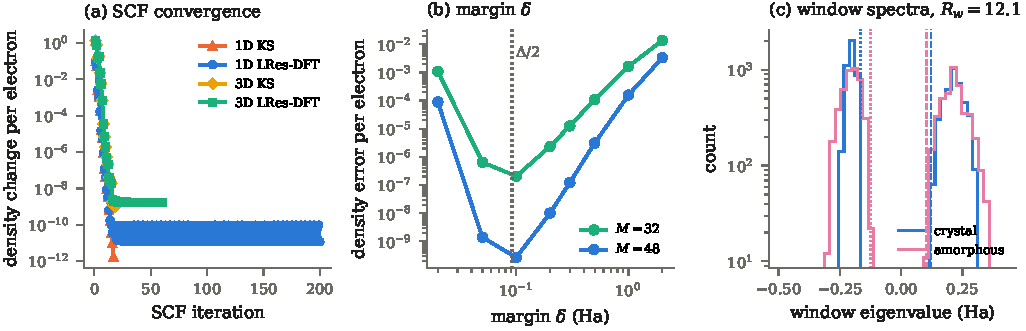
\includegraphics[width=\textwidth]{figures/figS1_supplement.pdf}
\caption{\label{fig:sm}(a)~SCF convergence of KS and LRes-DFT for a 1D (H$_2$)$_{16}$ chain and a 3D crystal with 128
electrons. (b)~Density error per electron of the 1D chain versus the margin $\delta$ for $M=32$ and 48; the dotted line marks
half the gap. (c)~Histogram of window eigenvalues at $R_w=12.1$~bohr for the crystal and the amorphous arrangement; dotted
and dashed lines mark the KS HOMO and LUMO.}
\end{figure}

% =============================================================================
\section{Verification and reproduction}\label{sec:repro}
% =============================================================================

\paragraph*{Computer algebra.} \texttt{cas\_verification.py} performs 30 checks with SymPy and 40-digit mpmath arithmetic:
\begin{itemize}
\item Lemma~1, for $M=2,\dots,14$ and as a matrix identity, including the non-orthogonal version;
\item the weight sum $\sum_j\zeta_j=0$;
\item Lemma~2: the Fermi--Dirac form in $\ln|u|$ and both bounds;
\item Proposition~1(b): the band energy from $g$;
\item the identity of Remark~2, symbolically and numerically;
\item Proposition~2: Jacobi's formula and the derivative of $W_M$;
\item the stationarity of $G_M$ at self-consistency, in a three-site model;
\item Proposition~3: $\partial\Omega_M/\partial\mu=-N_M$ for a rigidly moving circle;
\item Lemma~3: the recursion, symbolically for a $5\times5$ matrix;
\item Lemma~4: five random pencils;
\item the decay roots of the uniform-potential resolvent;
\item the LDA potentials as derivatives of the energy densities;
\item the pseudopotential Fourier transform;
\item the 1D exchange closed form against direct quadrature.
\end{itemize}
These checks verify the identities on explicit instances; the general proofs are in Appendix~A of the main text.

\paragraph*{Automated tests.} The 25 tests in \texttt{tests/} check:
\begin{itemize}
\item the recursion against dense inversion;
\item window convergence;
\item the closed form and occupation bounds against eigendecomposition;
\item the derivative identity by finite differences;
\item recovery of the diagonal of $h$;
\item the band energy against the eigenvalue sum;
\item a harmonic oscillator;
\item the exchange derivative;
\item self-consistent LRes-DFT against KS for four 1D systems;
\item 3D grid KS against dense diagonalization;
\item LCAO density normalization;
\item exactness of LRes-DFT when the window covers the cell;
\item 3D window convergence and self-consistency;
\item agreement of the C++ and Python implementations;
\item thread independence;
\item agreement of the six KS solver variants;
\item Lemma~4 on actual windows;
\item agreement of the stored-vector re-solution of $\mu$ with a full second pass.
\end{itemize}

\paragraph*{Scripts.} The data were produced by the following scripts:
\begin{itemize}
\item \texttt{benchmarks/accuracy.py}: exact two-electron and 1D KS comparisons;
\item \texttt{benchmarks/scaling.py}: 1D cost;
\item \texttt{benchmarks/extra\_checks.py}: grid refinement and grand-canonical forces;
\item \texttt{benchmarks/three\_d.py}: 3D accuracy, window and cost;
\item \texttt{benchmarks/referee\_checks.py}, parts R1--R18:
  \begin{itemize}
  \item DC comparison, compression, amorphous system, basis, margin, SCF histories;
  \item repeatability, memory, closing gap, pole rules, forces;
  \item window diagnostics and the Theorem~1 bound;
  \item occupation range, probing, LOBPCG, fixed-$N$ forces and threads;
  \end{itemize}
\item \texttt{benchmarks/scf3d\_large.py}: SCF up to 1024 electrons;
\item \texttt{benchmarks/ks\_drivers.py}: KS solver comparison.
\end{itemize}
Figures and tables are generated by \texttt{manuscript/make\_figures.py} and \texttt{manuscript/make\_tables.py}. The C++
kernels are built with \texttt{build\_cpp.sh}.

\end{document}
